\documentclass[10pt,twoside,draft]{book}
\usepackage{../../thesis}

\makeindex
\begin{document}

\chapter{Preliminaries: Topological Dynamical Systems}
\label{chap:prelim}
The purpose of this short chapter is to introduce notions of dynamical systems that will be used throughout the exposition.
The definitions that we present employ disparate sets of concepts, so those are introduced in respective chapters.

\begin{definition}
  (Dynamical System)
  Let $X$ be a topological space, and $F: X \to X$ be a continuous mapping.
  A (topological) dynamical system is defined to be a tuple $(X, F)$.
  %\index{}
\end{definition}
\begin{remark}
  We use a metric space as our topological space.
\end{remark}
%
\begin{definition}
  (Iteration)
  Let $F: X \to X$ be a mapping.
  \textit{The $n$-th iteration of F}, denoted $\itr{F}{n}$, is defined as follows
  \begin{equation*}
    \itr{F}{n} \ceq \underbrace{F \circ F \circ \cdots \circ F}_{n} .
  \end{equation*}
  Note that, if $F$ is continuous, then $\itr{F}{n}$ is continuous for any $n \in \N$.
\end{definition}
\begin{remark}
  We will never use the superscript notation to denote the exponentiation of a value of a function (as in $F(x) = 2x$, then $\itr{F}{2}(x) = 4x^2$).
\end{remark}
%%%
\begin{definition}
  (Orbit)
  Let $F: X \to X$. 
  The \textit{orbit} of $x_0$ is defined as the sequence
  \begin{equation*}
    O_F(x_0) \ceq \seq{\itr{F}{n}(x_0)}{\infty}{n = 0}.
  \end{equation*}
  $O_F(x_0)$ will simply be denoted as $O(x_0)$ when there is no ambiguity in the choice of $F$.
  \label{def:orbit}
  \index{orbit}
\end{definition}
%%%
It is convenient for our purpose to define the notion of a distance between a point and an orbit.
\begin{definition}
  (Metric of a point and an orbit)
  Let $X$ be a metric space, and $F: X \to X$ be a mapping.
  For each $x,y \in X$, the metric between $O(x)$ and $y$ is defined as follows
  \begin{equation*}
    \metric{O(x),y} \ceq \inf\limits_{x' \in O(x)} \metric{x',y}.
  \end{equation*}
\end{definition}
%%%
Now, we define two kinds of periodic behaviors.
Intuivitely speaking, periodic behaviors are tame behaviors that would not be associated with the term chaos.
However, chaotic and periodic behaviors are not at all mutually exclusive; as we will see, a dynamical system may have both of these elements.
\begin{definition}
  (Periodic point)
  Let $F: X \to X$ be a mapping, and $p$ be a point in $X$.
  If $\itr{F}{n}(p) = p$ for some $n > 0$, and $\itr{F}{m}(p) \neq p$ for each $1 \leq m < n$, then $p$ is called a \textit{periodic point} of period $n$, or simply a $n$-periodic point.
  \label{def:porbit}
  \index{periodic points}
\end{definition}
\begin{definition}
  (Asymptotically periodic point)
  Let $F: X \to X$ be a mapping, and $p$ be a point in $X$.
  $p$ is said to be a \textit{asymptotically periodic} point, if there exists a periodic point $q \in X$ such that
  \begin{equation*}
    \lim\limits_{n \to \infty} d(\itr{F}{n}(p), \itr{F}{n}(q))
    = 0.
  \end{equation*}
  \index{asymtotically periodic points}
\end{definition}
%%%
In topological dynamics, we are interested in properties that are preserved under continuous mappings.
All definitions of chaos that we discuss in the exposition are topological invariants.
%Since properties that we are specifically interested are global properties of a given space, we will require a conjugacy to be surjective. 
\begin{definition}
  (Conjugacy)
  Let $F: X \to X$ and $G: Y \to Y$ be continuous mappings.
  We say that $(X,F)$ is \textit{semi-conjugate} to $(Y,G)$ (by $\phi$), if there exists a continuous and surjective mapping $\phi: X \to Y$ such that $\phi\circ F = G\circ\phi$ (Figure~\ref{fig:conj}).
  Moreover, if $\phi: X \to Y$ is a homeomorphism, we say that $(X,F)$ is \textit{conjugate} to $(Y,G)$.
  \index{conjugacy}
\end{definition}
\begin{figure}[ht]
  \centering
  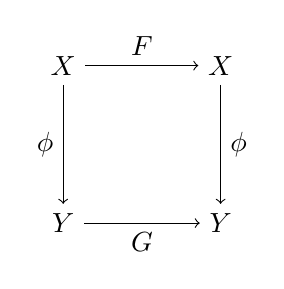
\begin{tikzpicture}[node distance=2cm, auto]
    \node (x1) {$X$};
    \node (x2) [right of=x1] {$X$};
    \node (y1) [below of=x1] {$Y$};
    \node (y2) [below of=x2] {$Y$};
    \draw[->] (x1) to node {$F$} (x2);
    \draw[->] (x1) to node[swap] {$\phi$} (y1);
    \draw[->] (y1) to node[swap] {$G$} (y2);
    \draw[->] (x2) to node {$\phi$} (y2);
  \end{tikzpicture}
  \caption{Conjugacy between $(X,F)$ and $(Y,G)$ by $\phi: X \to Y$.}
  \label{fig:conj}
\end{figure}
%%%
We often think of two dynamical systems as being ``the same'' when there exists a (homeomorphic) conjugacy between them, since they possess the same topological properties.

\bibliographystyle{../../pjgsm}
\bibliography{../../bibliography/thesis}

\printindex
\end{document}

%\section{Metric Spaces}
%This section introduces notations used in the rest of the book.
%Also, we prove the contraction fixed point theorem.
%
%\begin{definition}
%  (Metric space)
%  A binary operation $\metric{}$ is called a \textit{metric} if it satisfies the following properties for each $x,y,z \in X$:
%  \begin{enumerate}
%    \item $\metric{x,y} = 0 \mbox{ iff } x = y$
%    \item $\metric{x,y} = \metric{y,x}$
%    \item $\metric{x,y} \leq \metric{x,z} + \metric{z,y}$.
%  \end{enumerate}
%  A \textit{metric space} $X$ is a set equipped with a metric.
%  %\index{metric}
%\end{definition}
%%%
%\begin{definition}
%  (Neighborhood)
%  Let $X$ be a metric space, and $\delta$ be a metric on $X$.
%  For $\epsilon \in \R$, and $x \in X$, a (open) \textit{neighborhood} $\oball{\epsilon}{x}$ is defined as 
%  \begin{equation*}
%    \oball{\epsilon}{x} \ceq \setst{y}{\metric{y,x} < \epsilon}
%  \end{equation*}
%  I shall use the terms ``open ball'' and ``neighborhood'' interchangeably.
%\end{definition}
%%%
%\begin{definition}
%  (Closed neighborhood)
%  Let $X$ be a metric space, and $\delta$ be a metric on $X$.
%  For $\epsilon \in \R$, and $x,y \in X$, a \textit{closed neighborhood} $\cball{\epsilon}{x}$ is defined as the closure of the corresponding open neighborhood, i.e.
%  \begin{equation*}
%    \cball{\epsilon}{x} \ceq \cl(\oball{\epsilon}{x}).
%  \end{equation*}
%\end{definition}

%\begin{definition}
%  (Diameter of an set)
%  We denote the \textit{diameter} of $A \subseteq X$ by $\diam(A)$, and is defined as
%  \begin{equation*}
%    \sup\limits_{x,y \in A} \metric{x,y}.
%  \end{equation*}
%
%\end{definition}

%\begin{definition}
%  (Lipschitz constant; Contraction)
%  Let $X, Y$ be metric spaces, and $\delta_X$ and $\delta_Y$ be corresponding metrics.
%  A map $F: X \to Y$ is said to be a \textit{Lipschitz map} or to satisfy the \textit{Lipschitz condition} iff there exists a $C \in \R$ such that for each $x_1, x_2 \in X$,
%  \begin{equation}
%    \delta_Y(F(x_1),F(x_2)) \leq C \delta_X(x_1, x_2). 
%    \label{eqn:lipcond}
%  \end{equation}
%  Clearly, a Lipschitz map is uniformly continuous.
%  We define the \textit{Lipschitz constant}, $\Lip(F)$, of $F$ as the greatest lower bound of the set of all $C$, i.e.
%  \begin{equation*}
%    \Lip(F) \ceq \inf\setst{C}{C \mbox{ satisfies } \eqref{eqn:lipcond}}.
%  \end{equation*}
%  Furthermore, $F$ is called a \textit{contraction} if $\Lip(F) < 1$.
%  \index{Lipschitz constant}
%\end{definition}
%%%

%\begin{theorem}
%  (Contraction Fixed Point Theorem)
%  Let $(X,\delta)$ be a complete metric space, and $K: X \to X$ a contraction with $\Lip(K) = C$.
%  Then, $K$ has a unique fixed point.
%  \label{thm:cfp}
%  \index{contraction fixed point theorem}
%  %
%  \begin{proof}
%    For any point $x_0 \in X$, define
%    \begin{equation*}
%      x_n \ceq \itr{K}{n}(x_0).
%    \end{equation*}
%    We have
%    \begin{equation*}
%      \delta(x_{n+1}, x_n) \leq C \delta(x_n, x_{n-1}),
%    \end{equation*}
%    which implies
%    \begin{equation*}
%      \delta(x_{n+1}, x_n) \leq C^n \delta(x_1, x_0).
%    \end{equation*}
%    For any $m > n$, we have
%    \begin{align*}
%      \delta(x_m, x_n) &\leq \sum\limits_n^{m-1} \delta(x_{i+1}, x_i) 
%        \leq (C^n + C^{n+1} + \cdots + C^{m-1}) \cdot \delta(x_1, x_0) \\
%        & = C^n (C^{0} + \cdots + C^{m-n-1} ) \cdot \delta(x_1, x_0) \\
%        & = \frac{C^n(1 - C^{m-n})}{1-C} \cdot \delta(x_1, x_0)
%        \leq \frac{C^n}{1-C} \cdot \delta(x_1, x_0).
%    \end{align*}
%    Therefore, $\set{x_n}$ is Cauchy.
%    Since $X$ is complete, the sequence converges to a point in $X$, say $x$.
%    Finally, 
%    \begin{equation*}
%      K(x) = \lim\limits_{n\to \infty} K(x_n) = \lim\limits_{n\to \infty} x_{n+1} = x.
%    \end{equation*}
%    Thus, $x$ is a fixed point for $F$.
%  \end{proof}
%\end{theorem}
%%%

